\documentclass
[handout]
{beamer}
%\documentclass{beamer}

%%
%%
%%
% From http://tex.stackexchange.com/questions/2072/beamer-navigation-circles-without-subsections
% Solution #2 or 3:
% \usepackage{etoolbox}
% \makeatletter
% % replace the subsection number test with a test that always returns true
% \patchcmd{\slideentry}{\ifnum#2>0}{\ifnum2>0}{}{\@error{unable to patch}}%
% \makeatother
% Solution #1:
\usepackage{remreset}% tiny package containing just the \@removefromreset command
\makeatletter
\@removefromreset{subsection}{section}
\makeatother
\setcounter{subsection}{1}


\usepackage{etex}
\usepackage{pgf}
\usepackage{tikz}
\usepackage{url}
\usepackage{amsmath}
\usepackage{color}
% \definecolor{red}{rgb}{1,0,0}
\usepackage{ulem}
% \usepackage{booktabs}
\usepackage{colortbl,booktabs}
\renewcommand*{\thefootnote}{\fnsymbol{footnote}}
\usepackage{fancybox}
\usepackage[framemethod=TikZ]{mdframed}
\mdfdefinestyle{FactStyle}{%
  outerlinewidth=0.5,
  roundcorner=1pt,
  leftmargin=1cm,
  linecolor=blue,
  outerlinecolor=blue!70!black,
  backgroundcolor=yellow!40
}
\usepackage{cancel}

  \newcommand\Warning{%
    \makebox[2.4em][c]{%
      \makebox[0pt][c]{\raisebox{.2em}{\Large!}}%
      \makebox[0pt][c]{\color{red}\Huge$\bigtriangleup$}}}%

\usepackage{stackengine}
\usepackage{scalerel}
\usepackage{xcolor}
  \newcommand\dangersign[1][2ex]{%
    \renewcommand\stacktype{L}%
    \scaleto{\stackon[1.3pt]{\color{red}$\triangle$}{\tiny !}}{#1}%
  }



\usepackage{dcolumn}
\newcolumntype{d}[1]{D{.}{.}{#1}}

% From
% http://tex.stackexchange.com/questions/109900/how-can-i-box-multiple-aligned-equations
\usepackage{empheq}
\usepackage{tcolorbox}  \newtcbox{\othermathbox}[1][]{%
  nobeforeafter, tcbox raise base, 
  colback=black!10, colframe=red!30, 
  left=1em, top=0.5em, right=1em, bottom=0.5em}

\newcommand\blue{\color{blue}}
\newcommand\red{\color{red}}
\newcommand\green{\color{green!75!black}}
\newcommand\purple{\color{purple}}
\newcommand\bluegreen{\color{blue!75!green}}
\newcommand\orange{\color{orange}}
\newcommand\redgreen{\color{red!50!green}}
\newcommand\grey{\color{black}}
\newcommand\gap{\vspace{.1in}}
\newcommand\nb{${\red\bullet}\ $}
\newcommand\halfgap{\vspace{.05in}}
\newcommand\divideline{\line(1,0){352}}
\usepackage{marvosym} % for \Smiley

\newcommand{\bluealert}[1]{{\blue\textbf{#1}}}

% \usepackage{beamerthemesplit} %Key package for beamer
\usetheme{Singapore}
% \usetheme{Szeged}
% \usetheme{Garfield}
% \usetheme{CambridgeUS}
% \usenavigationsymbolstemplate{} %Gets rid of slide navigation symbols


\setbeamercolor{separation line}{use=structure,bg=structure.fg!50!bg}
% \begin{beamercolorbox}[colsep=0.5pt]
%   {upper separation line foot}
% \end{beamercolorbox}



\makeatletter
\setbeamertemplate{footline}
{
  \leavevmode%
  \hbox{%
% \begin{beamercolorbox}[colsep=0.5pt]
%   {upper separation line foot}
% \end{beamercolorbox}


  \begin{beamercolorbox}[wd=.5\paperwidth,ht=2.25ex,dp=2ex,colsep=0.5pt]%
    {upper separation line foot}
    \usebeamerfont{author in head/foot}%
    \hspace*{2ex}\insertshortdate:\ \insertshorttitle
  \end{beamercolorbox}%
  \begin{beamercolorbox}[wd=.5\paperwidth,ht=2.25ex,dp=2ex,right]{title in head/foot}%
    \usebeamerfont{title in head/foot}
    {\insertshortauthor}\hspace*{2ex}
  \end{beamercolorbox}}%
  % \begin{beamercolorbox}[wd=.333333\paperwidth,ht=2.25ex,dp=2ex,right]{date in head/foot}%
  %   \usebeamerfont{date in head/foot}\insertshortdate{}\hspace*{2em}
  %   \insertframenumber{} / \inserttotalframenumber\hspace*{2ex} 
  % \end{beamercolorbox}%
  \vskip0pt%
}
\makeatother

\usetikzlibrary{decorations.markings}
\usetikzlibrary{arrows}


\title{Final Exam Review}
\author{Peter Garfield, UCSB Mathematics}
\date{March 15, 2017}
%\institute{}


\useinnertheme{default}

\usefonttheme{serif}
% \usecolortheme{rose}
% \usecolortheme{whale}
% \usecolortheme{orchid}
\usecolortheme{crane}
% \usecolortheme{dolphin}


%TEMPLATE
\setbeamertemplate{navigation symbols}{}

\setbeamertemplate{note page}[compress]

\setbeamertemplate{frametitle}{
  \vspace{0.5em}
  % \begin{centering}
  {\huge\blue\textbf{\textmd{\insertframetitle}}}
  \par
  % \end{centering}
}

% From http://tex.stackexchange.com/questions/7032/good-way-to-make-textcircled-numbers:
\newcommand*\circled[1]{\tikz[baseline=(char.base)]{\node[shape=circle,draw,fill=orange,inner sep=1pt] (char) {#1};}} 
% \renewcommand{\labelenumi}{\circled{\textbf{\arabic{enumi}}}}

\let\olddescription\description
\let\oldenddescription\enddescription
\usepackage{enumitem}
\let\description\olddescription
\let\enddescription\oldenddescription

% \usepackage[loadonly]{enumitem}
\setlist[enumerate,1]{label=\colorbox{orange}{\arabic*.},font=\bfseries}
%\setlist[enumerate,2]{label=\colorbox{blue!25}{(\alph*)},font=\bfseries}
% \setlist[enumerate,1]{label=\arabic*.,font=\bfseries}
\setlist[itemize,1]{label=\red$\bullet$}
\setlist[itemize,2]{label=\blue$\bullet$}

\newcommand\answer[1]{\fbox{#1}}
% \renewcommand\answer[1]{}

\newcommand{\antilog}{\operatorname{antilog}}







\title{Word Problems, Inverse Functions, Pythagorean theorem!}
\date{March 31, 2022}


\begin{document}
\section{Introduction}
\frame{
  \frametitle{}
  {\Huge{}Welcome To Math 34A!}\\[.5em]

  {\Huge{}Differential Calculus}
  \vfill
  {\Large{}Instructor:}\\
  \ \hspace*{0.2in} Nathan Schley ({\it Sh}+{\it lye}), \url{schley@math.ucsb.edu}\\
  \ \hspace*{0.2in} South Hall 6701
  \\[0.5em]

  {\Large{}Office Hours:}\\
  \ \hspace*{0.2in} T R 11-11:50, T 3:45-4:35 Details on Gauchospace. 
  \bigskip

  \copyright\ 2017-22\ Daryl Cooper, Peter M.\ Garfield, Ebrahim Ebrahim \& Nathan Schley\\
  Please do not distribute outside of this course.
  \vfill

}

\frame{
  \frametitle{More travel problems}

  \begin{enumerate}
    \setcounter{enumi}{1}
  \item The Santa Barbara airbus leaves LAX at 3pm and drives to UCSB
    at an average speed of 30 mph.  You leave UCSB at 3pm driving at
    90 mph towards LAX. What time do you whiz past the airbus?
    \begin{center}
      A $=1\text{pm}$\quad 
      B $=3\text{:}30\text{pm}$\quad 
      C $=4\text{pm}$\quad
      D $=4\text{:}45\text{pm}$\quad
      E $=5\text{pm}$\quad
    \end{center}
    \pause
    \alert{Answer:}\ \answer{C}

    \medskip
    \pause

  \item  Same question/answers, but now you leave UCSB at {\red 4pm} 
    \smallskip
    \pause 
    
    \alert{Answer:}\ \answer{D}

  \end{enumerate}

}


%\frame{
%  \frametitle{Rectangle Problem}
%
%  \begin{enumerate}
%    \setcounter{enumi}{3}
%  \item A rectangle has {\red area $A$}, {\orange width $W$}, {\purple
%      length $L$} and {\blue perimeter $P$}.  \alert{Draw a picture}\
%    then work these out and {\blue i$>$click} as you do them.
%
%    \begin{itemize}
%    \item[(A)] Express {\red area} in terms of {\purple length} and
%      {\orange width}.
%      \bigskip
%
%    \item[(B)] Express {\purple length} in terms of {\red area} and
%      {\orange width}.
%      \bigskip
%
%    \item[(C)] Express {\blue perimeter} in terms of {\purple length}
%      and {\orange width}.
%      \bigskip
%
%    \item[(D)] Express {\orange width} in terms of {\blue perimeter} and
%      {\purple length}.
%      \bigskip
%
%    \item[(E)] Express {\red area} in terms of {\purple length} and
%      {\blue perimeter} 
%      \bigskip
%
%    \end{itemize}
%  \end{enumerate}
%
%}


\frame{
  \frametitle{Another Word Problem}

  \begin{enumerate}
    \setcounter{enumi}{3}
  \item Two numbers add up to give 17 and their product is 60. What is
    the larger of the two numbers?  
    \pause 
    \bigskip

    \alert{Method} / \alert{Plan}:\\
    \begin{itemize}
    \item[(i)] Name the two unknowns 
    \item[(ii)] create two equations 
    \item[(iii)] {\red solve} equations.
    \end{itemize}
    To {\red solve}: use one equation to eliminate one unknown from
    second equation, then factor the resulting quadratic.
    \bigskip

    \begin{center}
      A= I have answer\ \quad 
      B= working\quad 
      C=help
    \end{center}
  \end{enumerate}
}

\frame{
  \frametitle{Another one!}

  \begin{enumerate}
    \setcounter{enumi}{4}
  \item A rectangle has perimeter 34 inches and area 60 square inches.
    What is the length of the shortest side?
    \bigskip

    \begin{center}
      A= I have answer\ \quad 
      B= working\quad 
      C=help
    \end{center}
  \end{enumerate}

}





\section{Inverse Functions}

\frame{
  \frametitle{Inverse Functions}

  \alert{Idea:}\ 
  \parbox[t]{3in}{%
    You can plug in a power cord\\ \pause
    Inverse is to \colorbox{yellow}{\emph{unplug}}\ the cord.
  }
  \pause
  \bigskip
 
  \alert{Example:}\ 
  \parbox[t]{3in}{%
    $f(x) = 3x-2$ is a function of $x$ \\ \pause
    Inverse is $f^{-1}(y) = (y+2)/3$
  }
  \pause
  \vspace*{0.5in}

  \alert{General idea:}\ 
  \parbox[t]{3in}{%
    The inverse of $y=f(x)$ is $x=f^{-1}(y)$ \\ \pause
    Solve for $x$ in terms of $y$
  }
  \pause
  \bigskip 

  \alert{Example again:}\ 
  \parbox[t]{3in}{%
    $y = 3x-2$ is a function $f(x)$ \\ \pause
    Inverse is $x = f^{-1}(y) = (y+2)/3$
  }

}

\frame{
  \frametitle{More Examples}

  Try these, clicking as you go\ldots

  \begin{center}
    \begin{tabular}{cll}
      Click & \makebox[1in][l]{$y=f(x)$} & \makebox[1in][l]{$x=f^{-1}(y)$} \\ \toprule
      A & $y=5x$  &  $x = $\uncover<2->{$\,y/5$} 
      \\ \midrule
      B & $y=x+7$  &  $x = $\uncover<3->{$\,y-7$} 
      \\ \midrule
      C & $y=3x-4$  &  $x = $\uncover<4->{$\,(y+4)/3$} 
      \\ \midrule
      D & $y=x^3$  &  $x = $\uncover<5->{$\,\sqrt[3]{y} = y^{1/3}$} 
      \\ \midrule
      E & $y=2^x$  &  $x = $\only<6>{$\,$????}\only<7>{$\,\log_2(y)$} 
      \\ \bottomrule
    \end{tabular}
  \end{center}


}

\frame{
  \frametitle{Converting Temperature}
  \small

  ${\red x}=$ {\red temperature in Celsius}\qquad ${\blue y} = $ {\blue temperature in Fahrenheit}\ 
  \pause
  
  \gap 

  This table shows how to convert between  Fahrenheit and Celsius.

  \begin{table}
    \begin{tabular}{l*{11}{c}}
      \toprule
      ${\red ^oC}$ & {\red 0} & {\red 10}  & {\red \bf 20} & {\red 30} & {\red 40} & {\red 50} & {\red 60} & {\red 70} & {\red 80} & {\red 90} & {\red 100}\\
      ${\blue ^oF}$ & {\blue 32}  & {\blue 50}  & {\blue \bf 68} & {\blue 86} & {\blue 104} & {\blue 122} & {\blue 140} & {\blue 158} & {\blue 176} & {\blue 194} & {\blue 212}\\
      \toprule
    \end{tabular}
  \end{table}
  \pause

  There is a function $f$ that converts the temperature $\red x$ in
  Celsius to the temperature $\blue y$ in Fahrenheit: ${\blue
    y}=f({\red x})$
  \smallskip

  Example $f({\red 20})={\blue 68}$\quad means $\red {\bf 20}^oC$ is $\blue {\bf 68}^oF$\\
  \pause

  \gap
  The inverse function ${\red x}=f^{-1}({\blue y})$ converts
  Fahrenheit back into Celsius
  \pause

  Example: $f^{-1}({\blue 68})=\red 20$ 
  \pause

  \gap

  You can use a  table of data two ways:
  \begin{itemize}
  \item  Using it forwards gives you the function $f$
  \item  Using it backwards gives you the  inverse function $f^{-1}$
  \end{itemize}

}

\frame{
%  \frametitle{Find $f$ and $f^{-1}$ for Temperature}

    \begin{tabular}{l*{11}{c}}
      \toprule
      ${\red ^oC}$ & {\red 0} & {\red 10}  & {\red \bf 20} & {\red 30} & {\red 40} & {\red 50} & {\red 60} & {\red 70} & {\red 80} & {\red 90} & {\red 100}\\
      ${\blue ^oF}$ & {\blue 32}  & {\blue 50}  & {\blue \bf 68} & {\blue 86} & {\blue 104} & {\blue 122} & {\blue 140} & {\blue 158} & {\blue 176} & {\blue 194} & {\blue 212}\\
      \toprule
    \end{tabular}


  \small
  \begin{enumerate}
    \setcounter{enumi}{5}
  \item Find $y=f(x)$, the function that gives $y\,^{\circ}\text{F}$
    from $x\,{}^{\circ}\text{C}$.

    \begin{equation*}
      \text{A}\ y = 9x/5
      \quad 
      \text{B}\ y = 9(x+32)/5
      \quad 
      \text{C}\ y = (9x/5)+32
      \quad 
      \text{D}\ y = (9x+32)/5
    \end{equation*}
    \pause
    \alert{Answer:} \answer{C}      
    \bigskip
    \pause

  \item Find $x=f^{-1}(y)$, the function that gives $x\,^{\circ}\text{C}$
    from $y\,{}^{\circ}\text{F}$.

    \begin{equation*}
      \text{A}\ x = 5y/9
      \quad 
      \text{B}\ x = (5y+32)/9
      \quad 
      \text{C}\ x=(5y/9) + 32
      \quad 
      \text{D}\ x = 5(y-32)/9
    \end{equation*}
    \pause
    \alert{Answer:}\ \answer{D}      
    \bigskip
    \pause

  \item What temperature is the same in both Celsius and Fahrenheit?

    \begin{equation*}
      \text{A}\ -50^{\circ}
      \qquad 
      \text{B}\ -40^{\circ}
      \qquad 
      \text{C}\ -30^{\circ}
      \qquad 
      \text{D}\ -20^{\circ}
      \qquad 
      \text{E}\ -10^{\circ}
      \qquad 
      \pause
      \fbox{B}      
    \end{equation*}

  \end{enumerate}

}

\frame{
  \frametitle{Tax Table}
  \small
  \begin{table}
    \begin{tabular}{lllllll}
      \toprule
      Income 
      & {\blue\$$10,000\ \text{to}\ \$14,999$} 
      & {\red\$$15,000\ \text{to}\ \$19,999$} 
      & {\green\$$20,000\ \text{and over}$} 
      \\ 
      % \cmidrule[\heavyrulewidth](lr){1-1}
      \cmidrule[\heavyrulewidth](lr){2-2}
      \cmidrule[\heavyrulewidth](lr){3-3}
      \cmidrule[\heavyrulewidth](lr){4-4}
      %%%
                    & $\$600 +$  & $\$1,000 +$  &  $\$1,500+$ \\
      \text{Tax}    & $8\% \text{ of  amount }$ &  $10\% \text{ of  amount}$  & $12\%  \text{ of amount over}$  \\
                    & over {\blue$\$10,000$}    &  over {\red$\$15,000$}   &  over {\green$\$20,000$} \\
      \bottomrule
    \end{tabular}
  \end{table}

  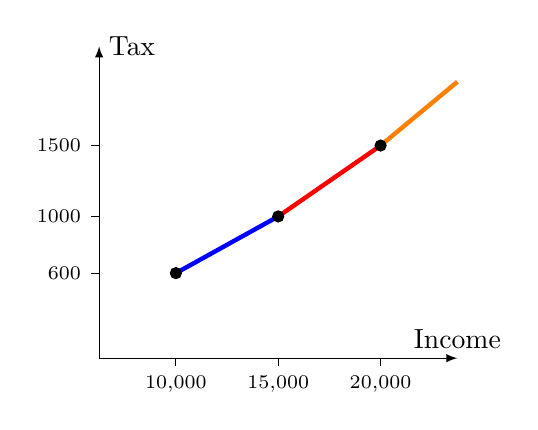
\begin{tikzpicture}[x=3.25mm,y=1.8mm,>=latex]
    \draw[thin,black,->] (0,0) -- (14,0) node[above] {Income};
    \draw[thin,black,->] (0,0) -- (0,22) node[right] {Tax};
    \foreach \y in {600,1000,1500} {
      \draw[thin,black] (0,{\y/100}) -- (-3pt,{\y/100}) node[left] {$\scriptstyle\y$};
    }
    % \foreach \x in {10000,15000,20000} {
      \draw[thin,black] (3,0) -- (3,-3pt) node[below] {$\scriptstyle10,000$};
      \draw[thin,black] (7,0) -- (7,-3pt) node[below] {$\scriptstyle15,000$};
      \draw[thin,black] (11,0) -- (11,-3pt) node[below] {$\scriptstyle20,000$};
    % }
    \draw[ultra thick,blue] (3,6) -- (7,10);
    \draw[ultra thick,red] (7,10) -- (11,15);
    \draw[ultra thick,orange] (11,15) -- (14,19.5);
    \filldraw[black] (3,6) circle (2pt);
    \filldraw[black] (7,10) circle (2pt);
    \filldraw[black] (11,15) circle (2pt);
  \end{tikzpicture}
  \qquad
  \parbox[b]{37.5mm}{%
    There are 3 {\purple tax brackets}
    \begin{center}
      {\blue 10K to 15K}\\
      {\red 15K to 20K}\\
      {\orange above 20K} 
    \end{center}
    \vspace{1in}
  }
  \vspace*{1.5in}

}


\frame{
  \frametitle{Tax, continued}
  \small
  \begin{table}
    \begin{tabular}{lllllll}
      \toprule
      Income 
      & {\blue\$$10,000\ \text{to}\ \$14,999$} 
      & {\red\$$15,000\ \text{to}\ \$19,999$} 
      & {\green\$$20,000\ \text{and over}$} 
      \\ 
      % \cmidrule[\heavyrulewidth](lr){1-1}
      \cmidrule[\heavyrulewidth](lr){2-2}
      \cmidrule[\heavyrulewidth](lr){3-3}
      \cmidrule[\heavyrulewidth](lr){4-4}
      %%%
                    & $\$600 +$  & $\$1,000 +$  &  $\$1,500+$ \\
      \text{Tax}    & $8\% \text{ of  amount }$ &  $10\% \text{ of  amount}$  & $12\%  \text{ of amount over}$  \\
                    & over {\blue$\$10,000$}    &  over {\red$\$15,000$}   &  over {\green$\$20,000$} \\
      \bottomrule
    \end{tabular}
  \end{table}

  \begin{enumerate}
    \setcounter{enumi}{8}
  \item If you earn \$$12,500$, how much tax do you pay?
    \qquad\qquad\qquad{\purple  read page 27} 
    \begin{equation*}
      \text{A}\ \$600
      \quad 
      \text{B}\ \$700
      \quad 
      \text{C}\ \$800
      \quad 
      \text{D}\ \$900
      \quad 
      \text{E}\ \$1,000
      \quad 
      \pause
      \fbox{C}
    \end{equation*}
    % \smallskip
    \vspace*{-2em}
    \pause
    \bigskip

    \item If you pay \$$1,200$\ in tax, how much do you earn?
      \begin{equation*}
        \text{A}\ \$16,000
        \quad 
        \text{B}\ \$17,000
        \quad 
        \text{C}\ \$18,000
        \quad 
        \text{D}\ \$20,000
        \quad 
        \pause
        \fbox{B}
      \end{equation*}
  \end{enumerate}
  % \smallskip
  \vspace*{1in}


}

\frame{
  \frametitle{Tax, continued some more}
  \small
  \begin{table}
    \begin{tabular}{lllllll}
      \toprule
      Income 
      & {\blue\$$10,000\ \text{to}\ \$14,999$} 
      & {\red\$$15,000\ \text{to}\ \$19,999$} 
      & {\green\$$20,000\ \text{and over}$} 
      \\ 
      % \cmidrule[\heavyrulewidth](lr){1-1}
      \cmidrule[\heavyrulewidth](lr){2-2}
      \cmidrule[\heavyrulewidth](lr){3-3}
      \cmidrule[\heavyrulewidth](lr){4-4}
      %%%
                    & $\$600 +$  & $\$1,000 +$  &  $\$1,500+$ \\
      \text{Tax}    & $8\% \text{ of  amount }$ &  $10\% \text{ of  amount}$  & $12\%  \text{ of amount over}$  \\
                    & over {\blue$\$10,000$}    &  over {\red$\$15,000$}   &  over {\green$\$20,000$} \\
      \bottomrule
    \end{tabular}
  \end{table}
  \bigskip


  If $x = \text{income}$ and $y = \text{tax}$, then
  \begin{itemize}
  \item $f(x)=y$ is the function with input income and output tax
    \medskip

  \item The inverse function $x=f^{-1}(y)$ has input tax and output income
    \medskip
  \end{itemize}
  \vspace*{2in}

}







\section*{Pyth Thm}

\small
\frame{
  \frametitle{\S1.7: Pythagoras' Theorem}

  \begin{minipage}{0.4\linewidth}
    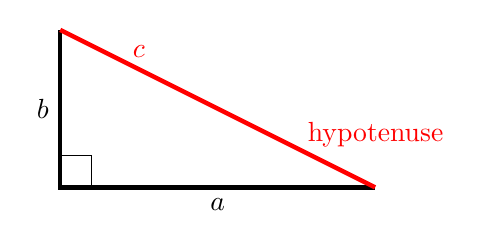
\begin{tikzpicture}[x=10mm,y=10mm,>=latex]
      \draw[ultra thick,black] (0,2) -- (0,0) node[midway,left] {$b$} -- (4,0) node[midway,below] {$a$};
      \draw[ultra thick,red] (0,2) -- (4,0) node[near start, above] {$c$} node[near end, right,
yshift=0.5em] {hypotenuse};
      \draw[thin,black] (0.4,0) -- (0.4,0.4) -- (0,0.4);
    \end{tikzpicture}
  \end{minipage}
  \begin{minipage}{0.55\linewidth}
    \begin{empheq}[box=\othermathbox]{align*}
      c^2 
      & = a^2 + b^2
    \end{empheq}
  \end{minipage}

  \begin{enumerate}
    \setcounter{enumi}{10}
  \item  What is the length of the hypotenuse of a right triangle when
    the other two sides have length ${\blue 3}$ and ${\blue 4}$? 

    \begin{center}
      A $=3$
      \quad 
      B $=4$
      \quad 
      C $=6$
      \quad 
      D $=25$
      \quad 
      E $=\text{none of these}$
      \pause 
      \quad
      \answer{E}
    \end{center}
    % They hypotenuse is length $5$!
    \smallskip
    \pause

  \item Now lengths are ${\blue 2}$ and ${\blue 3}$.  What's the hypotenuse?
    \begin{center}
      A $=\sqrt{5}$
      \quad 
      B $=\sqrt{13}$
      \quad 
      C $=13$
      \quad 
      D $=5$
      \pause
      \quad
      \answer{B}
    \end{center}
    \smallskip
    \pause

  \item Lengths ${\blue 3x}$ and ${\blue 4x}$. What's the hypotenuse?
    \begin{center}
      A $=5+x$
      \quad 
      B $=5x^2$
      \quad 
      C $=25x$
      \quad 
      D $=5x$
      \pause
      \quad
      \answer{D}
    \end{center}
  \end{enumerate}
  % This is \colorbox{yellow}{very useful}.

}


\frame{
  \frametitle{Pythagorean Theorem Applications}

  This is \colorbox{yellow}{very useful}\ to calculate how far apart two things are.
  \bigskip

  \begin{enumerate}
    \setcounter{enumi}{13}
  \item You and Marie are in Vegas. You drive north at 40 mph and
    Marie drives east at 30 mph.  How far apart are you after 1 hour?

    Click A when you have the answer.
    \pause
    \bigskip

  \item How many miles apart are you after $t$ hours? 
    \begin{center}
      A $= 50t$
      \quad 
      B $= 50+t$
      \quad 
      C $= 50t^2$
      \quad 
      D $= 2500t^2$
      \quad
      \pause
      \answer{A}
    \end{center}
    \bigskip
  \end{enumerate}


}


\frame{
  \frametitle{That's it. Thanks for being here. }

  \begin{center}
    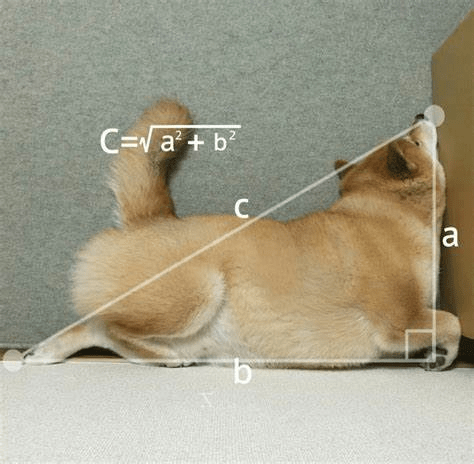
\includegraphics[scale=0.4]{Pyth_Doggie.png}
  \end{center}
}








\end{document}


%%% Local Variables: 
%%% mode: latex
%%% TeX-master: t
%%% End: 
